\documentclass[12pt]{article}
\usepackage{amsmath, amssymb, geometry, fancyhdr}
\usepackage{MnSymbol,wasysym}
\geometry{a4paper, margin=1in}
\setlength{\headheight}{15pt}
\pagestyle{fancy}
\fancyhf{}
\fancyhead[L]{CSCI-769 Quantum Computing Principles and Applications}
\fancyhead[R]{}
\fancyfoot[C]{\thepage}
\newcommand{\bra}[1]{\langle #1 |}
\newcommand{\ket}[1]{| #1 \rangle}
\usepackage{xcolor}
\usepackage{piton}
\usepackage{quantikz}
\usepackage{listings}

\lstset{
    language=Python,
    basicstyle=\ttfamily\small,
    keywordstyle=\color{blue},
    commentstyle=\color{green},
    stringstyle=\color{red},
    numbers=left,
    numberstyle=\tiny\color{gray},
    frame=single,
    breaklines=true,
    captionpos=b
}

\begin{document}

\title{CSCI-769 Quantum Computing Principles and Applications Homework 2}
\author{}
\date{}
\maketitle

\subsection*{1. Understanding The Effects Of Quantum Gates on Phase (10 pts)}

\textbf{Summary:} This explores how some single qubit gates impact the phase of a single qubit. These impact on phase lead to constructive and destructive interference between qubits during quantum algorithm execution which is one of the many reasons quantum algorithms are so powerful.
\begin{itemize}
    \item (a) Recall the phase shift gate  with parameter $\Tilde{\theta }$, $ P(\Tilde{\theta}) = \begin{bmatrix} 
1 & 0 \\ 
0 & e^{i\Tilde{\theta}} 
\end{bmatrix}$ , where $e^{i \Tilde{\theta}} = \cos(\Tilde{\theta}) +i\sin(\Tilde{\theta}) $. Find for the S,T, and Z gate what is the corresponding value of $\Tilde{\theta} $ that $P(\Tilde{\theta})$ yields the gate. 
\item b) Recall for on the Bloch Sphere $\ket{\psi} = \cos(\frac{\theta}{2}) \ket{0} +\sin(\frac{\theta}{2}) e^{i\phi} \ket{1} $, where $\phi$ is the phase. Report what happens to the phase of the quantum state when each gate is individually applied to the quantum state $\ket{\psi}$: X, S, T, and Z. Also report the phase shift for the Y gate as well. Hint: For the Y gate, $Y=iXZ$. Lastly figuring out what what value of $\Tilde{\theta}$ Euler's identity yields $i$, I promise this might be useful for this endeavor \smiley{}.
\end{itemize}






\subsection*{2. Phase and Measurement In the Standard Basis (10 pts)}

\textbf{Summary:} Ryan wants you to appreciate measurement in a more rigorous manner, and also understand how measurement is impacted by phase gates. This problem will explore the standard $\ket{0}, \ket{1} $ basis. 

(a) Apply an S-gate to $\ket{\psi} = \frac{1}{\sqrt{2}}( \ket{0} + \ket{1})$ e.g. $\ket{\phi_S} = S \ket{\phi}$. What is the resulting state in the computational basis?

(b)Measurement can be defined rigorously through inner products. For a state $\phi$, the probability of measuring basis state $\ket{j}$ is $P_j = |\langle j | \psi \rangle|^2 =   |\langle \psi | j \rangle|^2$. Use this definition to find probability of being in the $\ket{0}$ and $\ket{1}$ state respectively for both $\ket{\psi}$ and $\ket{\psi_S}$. Compare the measurements of being in the basis states for $\ket{\psi}$ and $\ket{\psi_S}$ - do they differ?

\subsection*{2. Phase and Measurement In the Hadamard Basis (10 pts)}

\textbf{Summary:} Ryan wants you to appreciate measurement in a more rigorous manner, and also understand how measurement is impacted by phase gates. This problem will explore the Hadamard Basis $\ket{+} = \frac{1}{\sqrt{2}} ( \ket{0} + \ket{1}) , \ket{-} =  \frac{1}{\sqrt{2}} ( \ket{0} - \ket{1}) $ basis.

(a) Apply an S-gate to $\ket{\psi} = \frac{1}{\sqrt{2}}( \ket{+} + \ket{-})$ e.g. $\ket{\phi_S} = S \ket{\phi}$. What is the resulting state in the computational basis?

(b)Measurement can be defined rigorously through inner products. For a state $\phi$, the probability of measuring basis state $\ket{j}$ is $P_j = |\langle j | \psi \rangle|^2 =   |\langle \psi | j \rangle|^2$. Use this definition to find probability of being in the $\ket{+}$ and $\ket{-}$ state respectively for both $\ket{\psi}$ and $\ket{\psi_S}$. Compare the measurements of being in the basis states for $\ket{\psi}$ and $\ket{\psi_S}$ - do they differ?

\subsection*{4. Getting some experience with the Toffoli (Controlled - Controlled X  - CCX) Gate (10 pts)}

\textbf{Summary:} On the journey from a quantum youngster to a quantum young adult, it’s vital to experience the challenge of calculating this circuit at least once. You’ll appreciate it later if you decide to eventually move from a quantum young adult to a rambling quantum old person like me \smiley{}.

Implement the Toffoli Circuit on the state $\ket{110}$ using two approaches. First, utilize the Toffoli circuit's matrix form to act on the state's vector representation to find what the Toffoli does to this state. Then, proceed to apply the circuit in stages, documenting the intermediate quantum states produced at each layer, until reaching the complete result of the Toffoli circuit applied to the state. Here is the Toffoli circuit picture
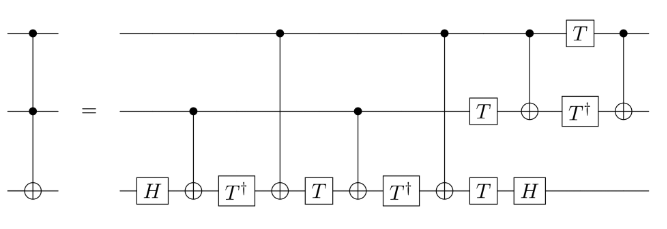
\includegraphics[]{toff.png}
and the matrix representation of the operator:

$\text{Toffoli} = \text{CCX} =
\begin{bmatrix}
1 & 0 & 0 & 0 & 0 & 0 & 0 & 0 \\
0 & 1 & 0 & 0 & 0 & 0 & 0 & 0 \\
0 & 0 & 1 & 0 & 0 & 0 & 0 & 0 \\
0 & 0 & 0 & 1 & 0 & 0 & 0 & 0 \\
0 & 0 & 0 & 0 & 1 & 0 & 0 & 0 \\
0 & 0 & 0 & 0 & 0 & 1 & 0 & 0 \\
0 & 0 & 0 & 0 & 0 & 0 & 0 & 1 \\
0 & 0 & 0 & 0 & 0 & 0 & 1 & 0
\end{bmatrix}.
$
Enjoy!

\subsection*{5. No-Cloning Theorem (10 pts)}

\textbf{Summary:} The no-cloning theorem is fundamental to quantum mechanics and prevents arbitrary quantum states from being copied. I think its great to prove it \smiley{} 

\[
\text{It is impossible to create an exact copy of an arbitrary unknown quantum state.}
\]

More formally, there does not exist a unitary operator \( U \) such that for an arbitrary quantum state \( |\psi\rangle \) and a fixed blank state \( |0\rangle \):

\[
U (|\psi\rangle \otimes |0\rangle) = |\psi\rangle \otimes |\psi\rangle, \quad \forall |\psi\rangle
\]
(a) Prove the no-cloning theorem mathematically: Hint assume the result is true and determine where a contradiction takes place. Recall since the matrix is unitary then $ U^*U=UU^*=I$. To help you get started:
\begin{itemize}
    \item 1. Consider two arbitrary quantum states \( |\psi\rangle \) and \( |\phi\rangle \).
\item 2. If cloning were possible, then for some unitary \( U \):

   \[
   U(|\psi\rangle \otimes |0\rangle) = |\psi\rangle \otimes |\psi\rangle
   \]

   \[
   U(|\phi\rangle \otimes |0\rangle) = |\phi\rangle \otimes |\phi\rangle
   \]

\item 3. Taking the inner product of these two equations with eacother, and follow what results using \[
\langle A \otimes B | C \otimes D \rangle = \langle A | C \rangle \langle B | D \rangle
\] to find the contradiction that the theorem would only hold for very specific quantum states, and not arbitrary quantum states
\end{itemize}

(b) While an arbitrary quantum state cannot be copied, there are two instances quantum state(s) can be copied. Write them down and explain why they can be copied.



\subsection*{7. Understanding the Impact Of Gate Failure Over A Long Period Of Time: Round 1 (10 pts)}

\textbf{Summary:} This question is designed to help everyone understand how such errors accumulate when quantum gates are applied multiple times. By analyzing how a small deviation in a Hadamard gate propagates over repeated applications, you can start to appreciate how quantum gate imperfections affect measurement probabilities (you could play this same game with any quantum gate - this question will give you the general idea though). The goal is to:

\begin{itemize}
    \item Understand how quantum errors accumulate over multiple gate applications.
    \item Analyze the deviation of a quantum state from its ideal evolution.
    \item Quantify the impact of errors on measurement probabilities.
    \item Recognize the necessity of quantum error correction in practical quantum computing.
\end{itemize}


In an ideal quantum circuit, quantum gates operate perfectly, ensuring that repeated applications of a gate yield the expected quantum state. However, in real-world quantum computers, quantum gates are subject to small errors due to hardware imperfections, decoherence, and noise. 

Consider the following scenario:

\begin{enumerate}
    \item A qubit is initialized in the state \( |0\rangle \).
    \item A Hadamard gate \( H \) is applied repeatedly \( n \) times. Ideally, applying \( H^2 \) should return the qubit to its original state: 
    \[
    H^2 |0\rangle = |0\rangle.
    \]
    \item However, assume each Hadamard gate has a small error represented by a unitary perturbation:
    \[
    H' = H + \epsilon U
    \]
    where \( U \) is some small deviation matrix and \( \epsilon \) is a small error factor.
    \item Over many applications, the accumulated error causes the final state to deviate from \( |0\rangle \). This impacts measurement probabilities.
\end{enumerate}

\textbf{Questions:}

\begin{enumerate}
    \item Show that if \( H \) were perfect, then applying \( H^2 \) to \( |0\rangle \) returns the state to \( |0\rangle \).
    \item Assume the error in \( H' \) propagates such that after \( n \) applications, the final state is:
    \[
    |\psi_n\rangle = (H')^n |0\rangle.
    \]
    Expand \( |\psi_n\rangle \) in terms of \( \epsilon \) and discuss how the error grows as \( n \) increases.
    \item Given that quantum measurements return \( |0\rangle \) with probability \( P(0) = |\langle 0 | \psi_n \rangle|^2 \), derive how this probability deviates from the expected value as a function of \( n \) and \( \epsilon \).
    \item Suppose \( \epsilon = 0.01 \) and \( n = 100 \). Numerically estimate the probability \( P(0) \) and discuss how this compares to the ideal case (\( P(0) = 1 \)).
    \item Based on your results, discuss why error correction techniques or fault-tolerant quantum computing are necessary for reliable quantum computation.
\end{enumerate}
\subsection*{8. Understanding the Impact Of Gate Failure Over A Long Period Of Time: Round 2 (10 pts)}
\textbf{Summary:} The goals here are the same as in Problem 7, but this time taking a closer look at how important phase errors impact constructive and destructive interference.

Consider the following scenario:

\begin{enumerate}
    \item A qubit is initialized in the state \( |+\rangle \), where:
    \[
    |+\rangle = \frac{1}{\sqrt{2}} (|0\rangle + |1\rangle).
    \]
    \item A phase gate \( P(\theta) \) is applied repeatedly \( n \) times, where the ideal phase gate is:
    \[
    P(\theta) = \begin{bmatrix} 1 & 0 \\ 0 & e^{i\theta} \end{bmatrix}.
    \]
    If \( P(\theta) \) is applied \( n \) times to \( |+\rangle \), the expected final state is:
    \[
    |\psi_n\rangle = \frac{1}{\sqrt{2}} (|0\rangle + e^{in\theta} |1\rangle).
    \]
    \item However, assume each phase gate has a small error represented by a unitary perturbation:
    \[
    P'(\theta) = P(\theta) + \epsilon U
    \]
    where \( U \) is some small deviation matrix and \( \epsilon \) is a small error factor.
    \item Over many applications, the accumulated phase error causes the final state to deviate from the expected state. This impacts constructive and destructive interference in measurement probabilities.
\end{enumerate}


\begin{enumerate}
    \item Show that if \( P(\theta) \) were perfect, then applying it \( n \) times to \( |+\rangle \) results in the state:
    \[
    |\psi_n\rangle = \frac{1}{\sqrt{2}} (|0\rangle + e^{in\theta} |1\rangle).
    \]
    Explain how constructive and destructive interference depends on \( n \theta \), e.g. calculate
    \begin{align*}
        P(+) = |\langle + | \psi_n \rangle \rangle|^2 \\ 
        P(-) = |\langle - | \psi_n \rangle \rangle|^2 
    \end{align*}
    
    \item Assume the error in \( P'(\theta) \) propagates such that after \( n \) applications, the final state is:
    \[
    |\psi_n\rangle = (P'(\theta))^n |+\rangle.
    \]
    Expand \( |\psi_n\rangle \) in terms of \( \epsilon \) and discuss how the phase deviation grows as \( n \) increases.
    
    \item Given that quantum measurements return \( |+\rangle \) or \( |-\rangle \) with probabilities:
    \[
    P(+) = |\langle + | \psi_n \rangle|^2, \quad P(-) = |\langle - | \psi_n \rangle|^2,
    \]
    derive how these probabilities deviate from their expected values as a function of \( n \) and \( \epsilon \).
    
    \item Suppose \( \epsilon = 0.01 \), \( \theta = \frac{\pi}{4} \), and \( n = 100 \). Numerically estimate the probability \( P(+) \) and discuss how this compares to the ideal case where \( P(+) \) is determined by perfect interference.
    
    \item Based on your results, discuss why error correction techniques or fault-tolerant quantum computing are necessary for reliable quantum interference-based computations.
\end{enumerate}
\subsection*{9. Implementing the SWAP Gate in Qiskit(10 pts)}

\textbf{Summary:} Recall \begin{equation*}
    SWAP_{01} = CNOT_{01}CNOT_{10}CNOT_{01},
\end{equation*}
which in circuit form looks like 

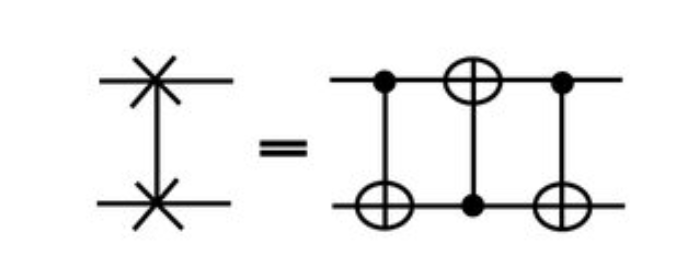
\includegraphics[scale=.5]{swap.png}

a) On paper write what the SWAP gate does to each of the four basis states.

b) For each basis state, run it with the AerSimulator (without noise) for 1000 shots each and report the counts for each run. Do your results agree with whats on paper?

d) For each basis state, execute it on a real IBM quantum computer with 100 shots and report those results.





\subsection*{9. Quantum Error Correction (10 pts)}

\textbf{Summary:} Quantum error correction is essential for fault-tolerant quantum computation.

(a) Implement the three-qubit bit-flip code in Qiskit.

(b) Simulate an error and demonstrate error correction.

\subsection*{10. Implementing The Toffoli In Qiskit (10 pts)}

\textbf{Summary:}This will get you exposed to the idea of state preparation, and implementing a more involved quantum circuit in Qiskit (to warm us up for the eventual Deutsch–Jozsa, Grover and Shor's circuits \smiley{})

a) Implement the Toffoli circuit (below) in Qiskit and apply it to all 8 basis states.
b) Before executing the Toffoli on a basis state, prepare the state using X gates (refer to why Ryan faced the Flip-ity Flop problem last homework \smiley{} - you were actually learning how to perform very basic state preparation!).
c) For each basis state, run it with the AerSimulator (without noise) for 1000 shots each and report the counts for each run.
d) For each basis state, execute it on a real IBM quantum computer with 100 shots and report those results.
e) Explain the impact that noisy intermediate scale hardware has on the theoretical predictions of the Toffoli applied to each basis state versus what is measured in each run. Research what the Toffoli gate should do to each of the 8 basis states to analyze each of the runs and understand how significantly noise affects measuring the "correct" answer.
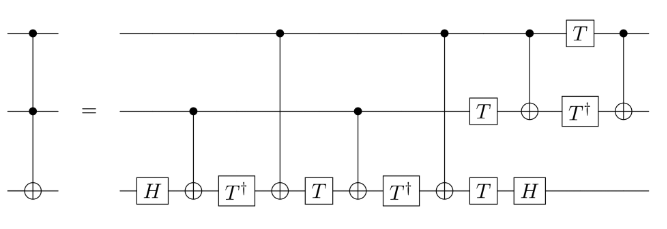
\includegraphics[]{toff.png}
\subsection*{Bonus Problem: Lindblad Master Equation (50 pts)}

\textbf{Summary:} The Lindblad master equation describes open quantum systems and their interactions with the environment. The mathematical objects involved are:
\begin{itemize}
    \item $\rho$ - The density matrix representing the quantum state (qubit) for a 2 level system, given by:
    \begin{equation*}
        \rho(t) = \begin{bmatrix} \rho_{00}(t) & \rho_{01}(t) \\ \rho_{10}(t) & \rho_{11}(t) \end{bmatrix},
    \end{equation*}
    where $\rho_{00}$ and $\rho_{11}$ represent the probabilities of measuring the system in the $|0\rangle$ and $|1\rangle$ states, respectively, and $\rho_{01}$ and $\rho_{10}$ represent coherence terms. In general this matrix is a $N \times N$ for a $N$ level system
    \item $\gamma$ - The decay rate associated with spontaneous emission.
    \item $\sigma_-$ and $\sigma_+$ - The lowering and raising operators, respectively, defined as:
    \begin{align*}
        \sigma_- &= \begin{bmatrix} 0 & 0 \\ 1 & 0 \end{bmatrix}, \quad
        \sigma_+ = \begin{bmatrix} 0 & 1 \\ 0 & 0 \end{bmatrix}.
    \end{align*}
    \item $\sigma_z$ - The Pauli-Z matrix:
    \begin{equation*}
        \sigma_z = \begin{bmatrix} 1 & 0 \\ 0 & -1 \end{bmatrix}.
    \end{equation*}
    \item $[A, B] = AB - BA$ - The commutator.
    \item $\{A, B\} = AB + BA$ - The anti-commutator.
    \item for a $N$ level system $\rho_{jj}$ is the probability at measurement you are in state $\ket{j}$.
\end{itemize}

\textbf{Initial Condition for an Uncertain State:} If the system is initially in an uncertain state, where it is in $|0\rangle$ with probability $p_0$ and in $|1\rangle$ with probability $p_1$ (such that $p_0 + p_1 = 1$), the initial density matrix is given by:
\begin{equation*}
    \rho(0) = p_0 |0\rangle \langle 0| + p_1 |1\rangle \langle 1| = \begin{bmatrix} p_0 & 0 \\ 0 & p_1 \end{bmatrix},
\end{equation*}
where $\ket{i}\bra{i}$ is an outer product. The \textbf{outer product} of a quantum state \( |\psi\rangle \) with itself, denoted as \( |\psi\rangle \langle \psi| \), is computed as follows:

1. Given a quantum state in column vector form:
   \[
   |\psi\rangle = \begin{bmatrix} a_1 \\ a_2 \\ \vdots \\ a_n \end{bmatrix}
   \]
   
2. Compute its conjugate transpose (bra):
   \[
   \langle \psi| = \begin{bmatrix} a_1^* & a_2^* & \cdots & a_n^* \end{bmatrix}
   \]

3. The outer product is given by:
   \[
   |\psi\rangle \langle \psi| =
   \begin{bmatrix} a_1 \\ a_2 \\ \vdots \\ a_n \end{bmatrix}
   \begin{bmatrix} a_1^* & a_2^* & \cdots & a_n^* \end{bmatrix}
   \]

   resulting in an \( n \times n \) Hermitian matrix:
   \[
   |\psi\rangle \langle \psi| =
   \begin{bmatrix}
   a_1 a_1^* & a_1 a_2^* & \cdots & a_1 a_n^* \\
   a_2 a_1^* & a_2 a_2^* & \cdots & a_2 a_n^* \\
   \vdots & \vdots & \ddots & \vdots \\
   a_n a_1^* & a_n a_2^* & \cdots & a_n a_n^*
   \end{bmatrix}
   \]

\textbf{Properties for the math nerds who are interested and want to do some further research:}
\begin{itemize}
    \item \( |\psi\rangle \langle \psi| \) is a \textbf{projection operator}.
    \item It is \textbf{Hermitian}: \( (|\psi\rangle \langle \psi|)^\dagger = |\psi\rangle \langle \psi| \).
    \item If \( |\psi\rangle \) is normalized, \( |\psi\rangle \langle \psi| \) represents a \textbf{pure state density matrix}.

\end{itemize}

For example, if there is uncertainty in the initial quantum state (or superposition) the quantum system is in e.g. $|0\rangle$ 50\% of the time and in $|1\rangle$ 50\% of the time, then:
\begin{equation*}
    \rho(0) = \frac{1}{2} \begin{bmatrix} 1 & 0 \\ 0 & 1 \end{bmatrix} = \begin{bmatrix} 0.5 & 0 \\ 0 & 0.5 \end{bmatrix}.
\end{equation*}
This represents a completely mixed state, indicating maximal uncertainty in the initial preparation.

(a) Solve analytically the Lindblad equation for a single qubit with spontaneous emission:
\begin{equation}
    \frac{d\rho}{dt} = -i[H, \rho] + \gamma (\sigma_- \rho \sigma_+ - \frac{1}{2}\{\sigma_+ \sigma_-, \rho\})
\end{equation}
where $H = \frac{1}{2} \sigma_z$ and $\gamma = 1$. Show that $P_0(t) + P_1(t) = \rho_{00}(t) + \rho_{11}(t)=1 $ : Hint Based on how you solve the problem this will be obvious, but in worst case, use the fact $\rho_{00}(0) +\rho_{11}(0)=1$. Lastly what happens to each one of these probabilities as $t \rightarrow \infty$?

(b) Use QuTiP to numerically solve this equation using 15000 time steps for $t\in[0,15]$, and using an initial condition above where 50 \% of the time the initial state is $\ket{0}$ and 50 \% of the time the initial state is $\ket{1}$ state. Plot  the numerical solutions for $\rho_{00}(t), \rho_{11}(t)$ and $\rho_{00}(t) + \rho_{11}(t)$. Also plot the the exact value of these quantities as found in a) to compare the numerical solutions with the analytical solutions. Do they agree?

\end{document}


\end{document}
